\documentclass[handout]{beamer}
\title[] % (optional, only for long titles)
{Algorithmic Verification of Channel Machines Using Small Models}
\author[J, Sharyari | \emph{sharyari@gmail.com}] {Jonathan Sharyari}
\usetheme{default}
\subject{Computer Science}

\usepackage{tikz}
\usetikzlibrary{arrows}
\usetikzlibrary{automata,positioning,shapes}

\newcommand{\petersonone}[1][]{
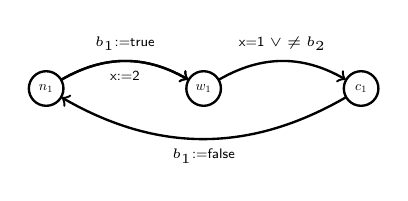
\begin{tikzpicture} [->,auto,node distance=2.0cm,line width=0.3mm]

  \node[state] (1) [scale=0.5]{$n_1$};
  \node[state] (2) [right of=1, scale=0.5] {$w_1$};
  \node[state] (3) [right of=2, scale=0.5] {$c_1$};

  \path[every node/.style={font=\sffamily\tiny}]
    (1) edge [bend left] node [above] {$b_1$:=true} (2)
    (1) edge [bend left] node [below] {x:=2} (2)
    (2) edge [bend left] node [above] {x=1 $\vee$ $\neq$ $b_2$} (3)
    (3) edge [bend left] node [below] {$b_1$:=false} (1);

\end{tikzpicture}
}




\newcommand{\petersontwo}[1][]{
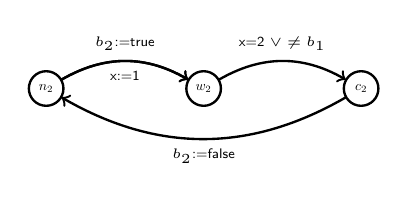
\begin{tikzpicture} [->,auto,node distance=2.0cm,line width=0.3mm]

  \node[state] (1) [scale=0.5]{$n_2$};
  \node[state] (2) [right of=1, scale=0.5] {$w_2$};
  \node[state] (3) [right of=2, scale=0.5] {$c_2$};

  \path[every node/.style={font=\sffamily\tiny}]
    (1) edge [bend left] node [above] {$b_2$:=true} (2)
    (1) edge [bend left] node [below] {x:=1} (2)
    (2) edge [bend left] node [above] {x=2 $\vee$ $\neq$ $b_1$} (3)
    (3) edge [bend left] node [below] {$b_2$:=false} (1);

\end{tikzpicture}
}



\newcommand{\petersonboth}[1][]{
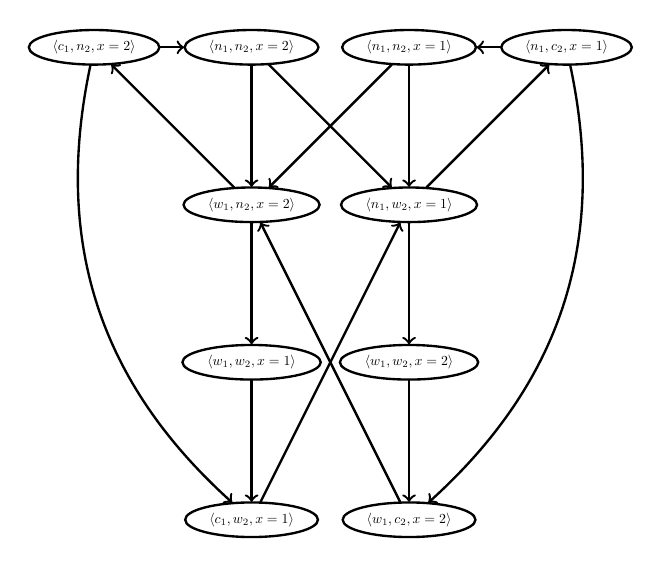
\begin{tikzpicture} [->,auto,node distance=2.0cm,line width=0.3mm]

  \node[state] (1) [ellipse,scale=0.5]{$\langle c_1,n_2,x=2\rangle$};
  \node[state] (2) [ellipse,right of=1, scale=0.5] {$\langle n_1,n_2,x=2\rangle$};
  \node[state] (3) [ellipse,right of=2, scale=0.5] {$\langle n_1,n_2,x=1\rangle$};
  \node[state] (4) [ellipse,right of=3,scale=0.5]{$\langle n_1,c_2, x=1\rangle$};
  \node[state] (5) [ellipse,below of=2, scale=0.5] {$\langle w_1,n_2,x=2\rangle$};
  \node[state] (6) [ellipse,below of=5, scale=0.5] {$\langle w_1,w_2,x=1\rangle$};
  \node[state] (7) [ellipse,below of=6, scale=0.5]{$\langle c_1, w_2,x=1\rangle$};
  \node[state] (8) [ellipse,below of=3, scale=0.5] {$\langle n_1,w_2,x=1\rangle$};
  \node[state] (9) [ellipse,below of=8, scale=0.5] {$\langle w_1,w_2, x=2\rangle$};
  \node[state] (10) [ellipse,below of=9, scale=0.5] {$\langle w_1,c_2,x=2\rangle$};


  \path[every node/.style={font=\sffamily\tiny}]
    (1) edge node [above] {} (2)
        edge [bend right] node [below] {} (7)
    (2) edge  node [below] {} (5)
        edge  node [below] {} (8)
    (3) edge node [above] {} (5)
        edge node [below] {} (8)
    (4) edge node [below] {} (3)
        edge [bend left] node [below] {} (10)
    (5) edge node [below] {} (6)
	edge node [below] {} (1)
    (6) edge node [below] {} (7)
    (7) edge node [below] {} (8)
    (8) edge node [below] {} (9)
	edge node [below] {} (4)
    (9) edge node [below] {} (10)
    (10) edge node [below] {} (5);



\end{tikzpicture}
}

\newcommand{\burns}[1][]{
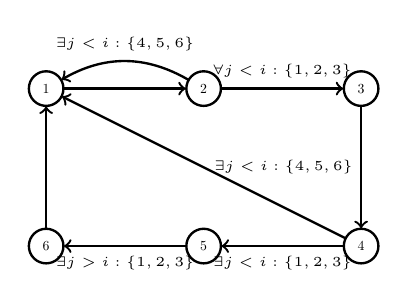
\begin{tikzpicture} [->,auto,node distance=2.0cm,line width=0.3mm]

  \node[state] (1) [scale=0.5]{$1$};
  \node[state] (2) [right of=1, scale=0.5] {$2$};
  \node[state] (3) [right of=2, scale=0.5] {$3$};
  \node[state] (4) [below of=3, scale=0.5] {$4$};
  \node[state] (5) [left of=4, scale=0.5] {$5$};
  \node[state] (6) [left of=5, scale=0.5]{$6$};

  \path[every node/.style={font=\sffamily\tiny}]
    (1) edge node [above] {} (2)
    (2) edge [bend right] node [above] {$\exists j<i: \{4,5,6\}$} (1)
     edge node [above] {$\forall j<i:\{1,2,3\}$} (3)
    (3) edge node [below] {} (4)
    (4) edge node [right] {$\exists j<i: \{4,5,6\}$} (1)
    (4) edge node [below] {$\exists j<i: \{1,2,3\}$} (5)
    (5) edge node [below] {$\exists j>i: \{1,2,3\}$} (6)
    (6) edge node [above] {} (1);
\end{tikzpicture}
}


\newcommand{\abpobserver}[1][]{
\begin{tikzpicture} [->,auto,node distance=3.0cm,line width=0.3mm]

%\begin{tikzpicture}[->,>=stealth',shorten >=1pt,auto,node distance=3cm,
%  thick,main node/.style={circle,fill=blue!20,draw,font=\sffamily\Large\bfseries}]

  \node[scale=0.5, state] (1) {$o_1$};
  \node[scale=0.5,state,accepting] (3) [right of=1] {$o_2$};
  \node[scale=0.5,state] (2) [right of=2] {$o_3$};

  \path[every node/.style={font=\sffamily\tiny}]
    (1) edge [bend left] node [above] {Snd} (2)
        edge node [above] {Rcv} (3)
    (2) edge [bend left] node [below] {Rcv} (1)
        edge node [above] {Snd} (3);
\end{tikzpicture}
}

\newcommand{\abpsender}[1][]{
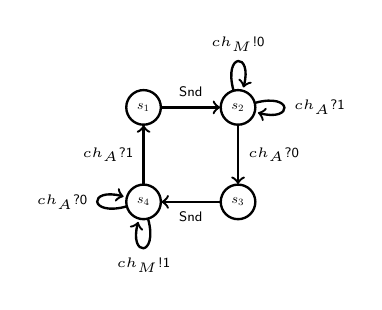
\begin{tikzpicture} [->,auto,node distance=2.4cm,line width=0.3mm]
  \node[scale=0.5,state] (1) {$s_1$};
  \node[scale=0.5,state] (2) [right of=1] {$s_2$};
  \node[scale=0.5,state] (3) [below of=2] {$s_3$};
  \node[scale=0.5,state] (4) [left of=3] {$s_4$};

  \path[every node/.style={font=\sffamily\tiny}]
    (1) edge node [above] {Snd} (2)
    (2) edge node [right] {$ch_A$?0} (3)
        edge [loop right] node {$ch_A$?1} (2)
        edge [loop above] node {$ch_M$!0} (2)
    (3) edge node [below] {Snd} (4)
    (4) edge node [left] {$ch_A$?1} (1)
        edge [loop left] node {$ch_A$?0} (4)
        edge [loop below] node {$ch_M$!1} (4);
\end{tikzpicture}
}

\newcommand{\abpreceiver}[1][]{
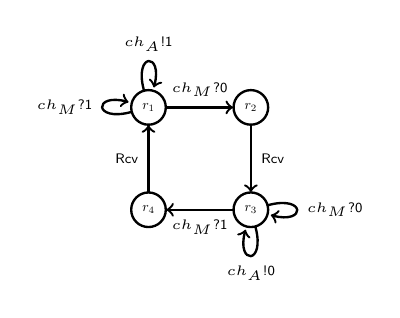
\begin{tikzpicture} [->,auto,node distance=2.6cm,line width=0.3mm]

  \node[scale=0.5,state] (1) {$r_1$};
  \node[scale=0.5,state] (2) [right of=1] {$r_2$};
  \node[scale=0.5,state] (3) [below of=2] {$r_3$};
  \node[scale=0.5,state] (4) [left of=3] {$r_4$};

  \path[every node/.style={font=\sffamily\tiny}]
    (1) edge node [above] {$ch_M$?0} (2)
        edge [loop left] node {$ch_M$?1} (1)
        edge [loop above] node {$ch_A$!1} (1)
    (2) edge node [right] {Rcv} (3)
    (3) edge node [below] {$ch_M$?1} (4)
        edge [loop right] node {$ch_M$?0} (3)
        edge [loop below] node {$ch_A$!0} (3)
    (4) edge node [left] {Rcv} (1);

\end{tikzpicture}
}


\newcommand{\abstraction}[1][]{
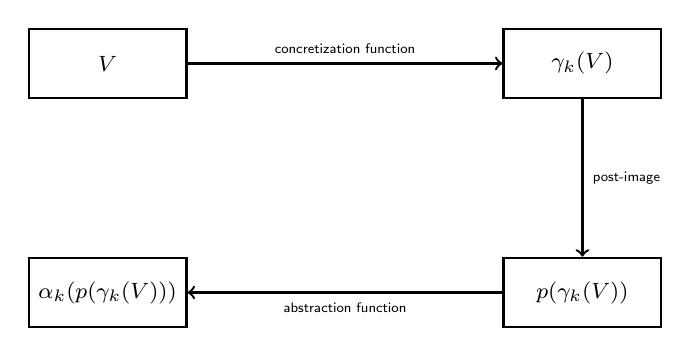
\begin{tikzpicture} [->,auto,node distance=2cm and 4cm,line width=0.3mm, font=\footnotesize]

  \node[state] (1) [rectangle, minimum width=2cm] {$V$};
  \node[state] (2) [rectangle, minimum width=2cm,right=of 1] {$\gamma_k(V)$};
  \node[state] (3) [rectangle, minimum width=2cm,below=of 2] {$p(\gamma_k(V))$};
  \node[state] (4) [rectangle, minimum width=2cm,left=of 3] {$\alpha_k(p(\gamma_k(V)))$};

  \path[every node/.style={font=\sffamily\tiny}]
    (1) edge node [above] {concretization function} (2)
    (2) edge node [right] {post-image} (3)
    (3) edge node [below] {abstraction function} (4);

\end{tikzpicture}
}


\newcommand{\freachability}[1][]{
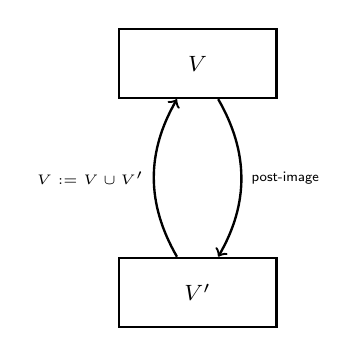
\begin{tikzpicture} [->,auto,node distance=2cm and 4cm,line width=0.3mm, font=\footnotesize]

  \node[state] (1) [rectangle, minimum width=2cm] {$V$};
  \node[state] (2) [rectangle, minimum width=2cm,below=of 1] {$V'$};

  \path[every node/.style={font=\sffamily\tiny}]
    (1) edge [bend left] node [right] {post-image} (2)
    (2) edge [bend left] node [left] {$V := V \cup V'$} (1);
\end{tikzpicture}
}

\date[2014-09-09] % appears in the bottom of the sidebar
{September $9^{th}$, 2014}
\institute[Dept.\ of Information Technology]
{Department of Information Technology\\
  Uppsala University \\ \vspace{10pt}
  Supervisor: Parosh Abdulla \\
  Reviewer: Mohamed Faouzi Atig}
\usepackage{float}
\newfloat{algorithm}{t}{lop}
%\usepackage{subfigure}
\usepackage{subcaption}
\usepackage{algpseudocode}
\usepackage{biblatex}
%\addbibresource{references.bib}
\algtext*{EndWhile}% Remove "end while" text
\algtext*{EndIf}% Remove "end if" text
\algtext*{EndFor}% Remove "end if" text
\begin{document}
\begin{footnotesize}
\begin{frame}[plain]
My name is Jonathan Sharyari, I'm an IT student here at Uppsala university, and I'm going to present my master thesis, ``algorithmic verification of channel machines using small models''. This is an internal project for the algorithmic program verification group, with Parosh Abdulla as supervisor and Mohamed Faouzi Atig as reviewer.
\end{frame}

\begin{frame}
\begin{itemize}
\item
This is an outline of my speech: I will start by explaining some general concepts of verification, with some small examples, unrelated to my work. I then continue with some more specific terminology related to what I do, but in another context. There's two reasons for this: the first is that my goal of my master thesis was to adapt an exisiting approach to a new setting, and therefore I first present the work on which mine is based, and second, examplifying the concepts gets much less cluttered.
\item
Thereafter, I will explain what my task was, the adaptions I've did and the difficulties I had to face, and to round off, I show some results in comparison to some other approaches to solve the same problem.
\end{itemize}
\end{frame}


\section{General Verification}
\subsection*{1}
\begin{frame}
  \frametitle{Verification}
  \begin{itemize}
  \item
  In general, verification is the ``process of evaluating software to determine whether the products of a given development phase satisfy the conditions imposed at the start of that phase''. In this context the term verification refers to ``formal verification'' or ``algorithmic verification'', i.e.\ to formally either prove or disprove the correctness of algorithms.
  \item
  With the term model checking, I refer to the task of performing automated verification of algorithms: in general, one specifies the behaviour of the algorithm as a graph, and specifies either the desired or the undesired behaviour of the algorithm, and then performs an exhaustive search in the graph. The exhaustive search corresponds in essense to all the possible outcomes of the algorithm, and the algorithm is safe, if all possible outcomes exhibit the desired behaviour.
  \item
  A common way to describe the intended or unintended behavior is to use linear time logic, and this more specific approach is often simply called ``model checking''; This is not the approach used in this project, and I'm mentioning this to avoid potential confusion.
  \end{itemize}
\end{frame}

\subsection*{1}
\begin{frame}
  \frametitle{Peterson's Mutual Exclusion -- Pseudo Code}
As an example of verification, we take a simple algorithm, peterson's mutual exclusion algorithm. The goal is that two processes communicate over shared variables in order to avoid that both processes are in their critical section at the same time. We can describe this algorithm as a graph, which would look like this:
\end{frame}

\subsection*{1}
\begin{frame}
\begin{itemize}
\item
The two processes have one graph each, rather similar in this case, with three local states each, n1, w1, c1, n2,w2 and c2, where n means non-critical, w means waiting and c is the critical section. From these two graphs, we can see that the unintended behaviour would be that P1 would be in state c1 at the same time as P2 would be in state p2, but neither c1 nor c2 is a bad state in itself.
\item
We need a graph that describes the joint behaviour of the two program graphs, in order to express the bad state, before we can prove or disprove the existence of such a bad state.

\end{itemize}
\end{frame}

\subsection*{1}
\begin{frame}
  \frametitle{Peterson's Mutual Exclusion -- Transition System}
\begin{itemize}
\item
For this, we use a transition system. This graph shows all the reachable states of the transition system corresponding to the two program graphs. Each node in the graph is a global state, which is in turn described by the local state of P1, the local state of P2, and the value of the shared variable x, which can be either 1 or 2. Since no node has both P1 and P2 in their critical sections, petersons mutual exclusion algorithm is safe. There are several methods to find the reachable set of states, in this case, forward reachability analysis is enough: basically, start in the initial state, and take all possible combinations of action.
\item
This approached works fine for this simple algorithm, there being only two processes. But what would happen if we would do the same thing for a mutual exclusion algorithm without an upper bound on the number processes using it? This would mean that we would have an infinite number of program graphs, and a transition system like the one here, where would be a subset of all the combinations of their local states. An exhaustive search in such a graph would of course be infeasible.
\end{itemize}
\end{frame}


\section{All for the Price of Few}
\subsection*{1}
\begin{frame}
  \frametitle{All for the Price of Few}
  \begin{itemize}
\item
One approach to solving this problem was presented in the paper ``all for the price of few'', written Parosh Abdulla, my supervisor, Frederic Haziza and Lukas Holik, published last year. I will in short present their results, in order to explain some additional techniques and terminology: paramterized system, small models and view abstrabction.
  \end{itemize}
\end{frame}

\subsection*{1}
\subsection{Parameterized Systems}
\begin{frame}
  \frametitle{Parameterized Systems}
  \begin{itemize}
  \item
  Parameterized system are systems, where the size of the system is a parameter of the system itself. A mutual exclusion algorithm with unbounded number of participants is one example, and as I mentioned, it results in an infinite size system. This happens not only when there is an unbounded number of participents, but as soon as any global artifact becomes unbounded, for example an integer counter, or communication over unbounded channels.

  \end{itemize}
\end{frame}

\subsection*{1}
\begin{frame}
  \frametitle{Parameterized Systems -- Burns' Protocol}
\begin{itemize}
\item
Here we see a mutual exclusion algorithm with unbounded number of participents, the burns' protocol. Each protocol has the exact same program graph, with 6 local states where the 6:th one represents the critical section. How this works exactly is not that important in this context.

\end{itemize}
\end{frame}


\subsection{Small Models}
\begin{frame}
  \frametitle{Small Models}
  \begin{itemize}
  \item
As the verification on inifite systems is impossible, we must somehow make the problem finite. A simple method would then to simply put a limit on the number of participents, lets say 5. But proving that the system is safe when there are 2, 3, 4 or 5 processes, is not really a proof that it will still be safe for 6,7 or 8 participents.
\item
    The underlying idea to solve this, is the concept of ``small models''. In some cases, it turns out that it is possible to find a ``small model'', that exhibits all the relevant behaviour of larger models. If we can prove that what we are verifying actually does exhibit all the relevant behaviour of larger models, then proving the correctness for 5 processes will indeed be a proof for any larger size as well.

  \end{itemize}
\end{frame}

\subsection{View Abstraction}
\begin{frame}
\frametitle{View Abstraction} % mention ``Abstract interpretation''

\begin{itemize}
\item
The question then, is how to show that a certain problem instance is actually a small model. To do this, they use a technique called view abstraction, which is a type of abstract interpretation. Graphically, the process looks something like this:
\item
Instead of only calculating the set of reachable global states, we also create an over-approximation of that set using what we we call a concretization function and a an abstraction function. The upper left box is marked V, which is a set of views, up to a certain size k. The concretization function takes the this set, and finds a set gamma of configurations of size k+1. You could think of this as a set of reachable states, if there would have been yet another process in the system. Then we take the post-image of this set, which means that we see which other configurations of size k+1 are reachable from the set gamma k. From this set of configurations of size k+1, we use an abstraction function to reduce this to a set of corresponding views of size k.
\end{itemize}
\end{frame}

\begin{frame}
Drawing example
\end{frame}

\subsection{Verification Algorithm}
\begin{frame}
  \frametitle{Verification algorithm} % mention ``Abstract interpretation''
\begin{itemize}
\item
This results in a verification algorithm, that looks a bit like this. It has two distinct parts: the first part is to use some verification technique to check whether a finite model is safe or not, using any technique: this could be for example forward reachability. The second part consists of applying the concretization function gamma and abstraction function alpha, trying to show that the model is a small model.
\item
To be a bit more precise, I'll step through the algorithm once. We start with the smallest number k of participents, in the case of mutual exclusion algorithms, that would be 2.  In the first step, we find the reachable set of global states, such as we saw for peterson's algorithm earlier, and check if any of those states is a bad state. If such a state exists, we have shown that the algorithm is unsafe, and we're done.
\item
If not, we want to check if k=2 is a small model. We apply the concretization and abstraction function, and create the overapproximation of reachable configurations, and check whether any of those configurations is a bad configuration. If we do find such a bad configuration, we havn't shown that the algorithm is unsafe, but merely that that specific instance of the algorithm with 2 participents is not a small model, therefore we add yet another participant, i.e.\ we use a larger model, and repeat again.
\end{itemize}

\end{frame}

\section{Objective}
\subsection*{1}
\begin{frame}
  \frametitle{Goal}
  \begin{itemize}
    \item
You have probably noticed that I still havn't explained what my thesis work is about. Recall that parameterized systems arise, when there is some unbounded entity within a system, leading to an infinite system. One example was an unbounded number of processes, and solving this problem was the goal of this paper by the Algorithmic Program Verification group. Another example was the presence of unbounded integers, and solving this problem was the topic of another master thesis this year by Thomas Sävström. The last example was the presence of unbounded buffers, and this is the topic of my master thesis.
\item
My task was to adapt the model that I have presented, to a method of verifying channel systems, i.e.\ systems working with unbounded buffers. Perhaps a bit oversimplified, this means that I'm using the same verification algorithm as we just saw, but with other functions for alpha and gamma.
\item
The difficulty is then, to define a concretization function gamma and an abstraction function alpha, and to prove that the continuous application of these function will indeed result in the proof of a small model.
\item
The second part of the task was to implement the verification method, the difficulty of which is of course trying to do efficiently.
  \end{itemize}
\end{frame}

\begin{frame}
\begin{itemize}
\item
In the remaining time, I'm going to explain more precisely what I mean with a channel system, and give an example for it. I will also shortly define the functions alpha and gamma, just enough to give an intuitive feeling for it. These functions are the most central point of what I have been working on, so it's only fair that I show them, but they are a bit to messy for me to explain adequately withing the short time frame I have.
\item
And last, I will compare the results of my work to two other methods for solving the same problem, and apply some self-critisism.
\end{itemize}
\end{frame}


\section{Method}
\subsection{Channel Systems}
\begin{frame}
  \frametitle{Channel Systems}
  \begin{itemize}
  \item
So a channel system is any system that relies on channels for its operation, the most typical example being communication protocols, where the participants have an ingoing and outgoing buffer for their communication.
\item
Without an upper bound on the size of the buffers, the transition system that would need to be examined would be an infinite graph.
    \end{itemize}
\end{frame}

\subsection*{1}
\begin{frame}
\frametitle{ABP -- Program Graphs}
\begin{itemize}
\item
Here's one of the simplest examples of a communication protocol, the alternating bit protocol. There is a sender to the left and a receiver to the right, with four local states each. There are two communication buffers: the sender sends messages on the channel M, and the receiver sends acknowledgements back to the sender, when it receives a message. In this case, the actual messages being sent have been abstracted away, because the actual content doesn't affect the functionality. Instead, they are only sending either a message marked with 0, or marked with 1. This is the ID of the message, and the idea is that the ID alternates between 0 and 1. The goal of the protocol is that the receiver should receive all its messages in the correct order.
\item
So the two program graphs a and b represent the protocol itself, but additionally, I have a third component called an observer. This is a modeling artifact, with the sole functionality that it allows me to capture what a bad state is: Each time the sender sends a new message, the observer follows one of the arcs marked with snd, and when the receiver receives a new message, the observer follows an arc marked rcv. A bad event is, if the sender manages to send two messages with different ID numbers, without the receiver receiving a message in between these events, and vice versa. This means that the bad state of this protocol is $o_2$ in the observer.
\end{itemize}
\end{frame}

\subsection{Transition System}
\begin{frame}
  \frametitle{Channel Transition System}
  \begin{itemize}
  \item
The corresponding transition system is a system describing the joint functionality of the three processes. In the case of peterson's mutual exclusion before, that was the local state of the two processes and the state of the shared variable x. In this case, it is the local states of the three processes, and the states of the shared buffers channel M and channel A. Peterson's algorithm had a transition system with ten reachable states, ABP has 108 reachable states, so drawing it is not really an option.
\item
We say that each state is a tuple S, and xi, where S is the global state of the three processes, and xi is the state of the channels, which I call the evaluation as not to overload the term.
  \end{itemize}
\end{frame}

\subsection{$\alpha$ and $\gamma$}
\begin{frame}
\begin{itemize}
\item
The point of view abstraction was, that for a system of a certain size k, in this case the size means the size of the buffers, to show that that system is indeed a small model. The technique was to create an overapproximation of states, by repeatedly applying a concretization function and an abstraction function. In this graph, V is this overapproximation of states. The concretization function creates configurations of size $k+1$, i.e.\ of larger size than the buffer can have, the post-image simply follows an an arc in the program graphs, and the abstraction functions reduces the result back to something of size $k$, and this will be the new set V in the next iteration. If the new set V is the same as the old set V, we have reached a fixpoint.
\end{itemize}
\end{frame}

\subsection*{1}
\begin{frame}
  \frametitle{Abstraction Function}
  \begin{itemize}
  \item
  In the example before, the abstraction function was the set of subwords of a word. In the case of channel systems, the abstraction function is the subwords of the channel evaluations. Since there may be several channels in the system, it becomes the cross product of all the subwords of all the channels.
\item
  Take the alternating bit protocol as an example. The subwords of size 2 of 110 are 11, 10, 1, 0 and empty word. The subwords of 0 are 0 and empty word. In total, we get 2*5 = 10 views. Calculating the views of a configuration is rather straight forward.

    \end{itemize}
\end{frame}

\subsection*{1}
\begin{frame}
  \frametitle{Concretization function}
  \begin{itemize}
  \item
  The concretization function goes in the opposite direction, but is far more difficult to calculate in practice.

  \item
  Using the same input as before, we not only get back [110,0] that we started with, but also three additional configuration, because the different subsets of the inputs are the views of these configurations.
\item
  This is one of the main difficulties that needed to be overcome, in order to write an efficient information. In this example, the input is only 10 views, resulting in 4 configuration. If we look at the verification results from some algorithms, we see in the second column that the number of views range between 45 and 1,8 million, and how to compute this becomes somewhat cumbersome.
  \end{itemize}
\end{frame}


\section{Results}
\begin{frame}
  \frametitle{Statistics}
  \item
    This table shows the verification results for a few communication protocols: abp is the alternating bit protocol that we saw earlier, whereas sw stands for the sliding window protocol and the number denotes window size, 3, 4 and 5 in this case, and brp is the bounded retransmission protocol. The last three protocols are the same, but with deliberate faults added to the protocols in order to make them unsafe.
    \item
    The columns show the verification results with three different verifiers, the first being the one I've implemented for my thesis. I have also implemented a second verifier, using backward reachability, based on a paper by Parosh from 1993. The last verifier, MPass is a verifier from the apv group, which basically translates verification problems to satisfiability problems, and uses third party SAT solvers to solve them.
    \item
    I would read too much into this small set of tests, but what can be said is, first that the results seem to be correct, second that for the most part, the verifier performs well in comparison. But this also highlights the main drawback of this method: overapproximation of states lead to quite a lot of states. Looking at sliding window with a window size of 5, we see from the backward reachability that there are 2028 reachable states, but the number of configurations when overapproximating is over 1,8 million.
\end{itemize}
\end{frame}

\end{footnotesize}
\end{document}
